%------------------------------------------%
%
% Cannabis Data Science #66
%
% Date: 5/18/2022
%
%------------------------------------------%
\documentclass[xcolor={dvipsnames}]{beamer}
\hypersetup{pdfpagemode = FullScreen}
\mode<presentation>{
  \usetheme{Boadilla}
  \usecolortheme{orchid}
  \usefonttheme{default}
  \setbeamertemplate{navigation symbols}{}
  \setbeamertemplate{caption}[numbered]
}
\setbeamersize{
  text margin left = 0.5in,
  text margin right = 0.5in
}

%------------------------------------------%
% Title
%------------------------------------------%
\title[\textbf{Cannabis Data Science \#65}]{}
\author{Cannlytics}
\institute[]{\Large Cannabis Data Science \#65}
\date{May \nth{11}, 2022}

%------------------------------------------%
% Packages
%------------------------------------------%
\usepackage[english]{babel}
\usepackage[utf8x]{inputenc}
\usepackage{tikz} % For styling.
\usepackage{xparse}

%------------------------------------------%
% Colors
%------------------------------------------%
\definecolor{Green}{RGB}{34, 153, 84}
\definecolor{LightGreen}{RGB}{218, 247, 166}
\definecolor{DarkGreen}{RGB}{2, 48, 32}
\definecolor{Orange}{RGB}{255, 87, 51}
\definecolor{DarkOrange}{RGB}{199, 0, 57}
\definecolor{Yellow}{RGB}{255, 195, 0}

%------------------------------------------%
% Theme
%------------------------------------------%
\setbeamercolor*{palette primary}{bg=LightGreen, fg=DarkGreen}
\setbeamercolor*{palette secondary}{bg=LightGreen, fg=DarkGreen}
\setbeamercolor*{palette tertiary}{bg=LightGreen, fg=DarkGreen}

%------------------------------------------%
% Packages
%------------------------------------------%
\usepackage{amsmath}
\renewcommand*\footnoterule{} % No separating line on footnote.
\usepackage{mathtools} % For annotating equations.
\usepackage{hhline} % for double bars.
\usepackage[super]{nth} % For formatting 1st, 2nd, 3rd, etc.
\usepackage{graphicx, caption, subcaption}
\usepackage{setspace}
\usepackage[charter]{mathdesign}
\usepackage{tikz}
\usetikzlibrary{tikzmark}
\usetikzlibrary{arrows.meta}

%------------------------------------------%
% Commands
%------------------------------------------%

% Top space.
\newcommand\T{\rule{0pt}{2.5ex}}

% Bottom space.
\newcommand\B{\rule[-1.25ex]{0pt}{0pt}}

% Blocks.
\newenvironment<>{Block}[2][.9\textwidth]
  {\setlength{\textwidth}{#1}
  \begin{actionenv}#3
    \def\insertblocktitle{#2}\par
    \usebeamertemplate{block begin}}
  {\par\usebeamertemplate{block end}
  \end{actionenv}}

% Balls.
\defbeamertemplate{enumerate item}{largeball}
{\begin{pgfpicture}{-1ex}{-0.65ex}{1.5ex}{1.5ex}
\usebeamercolor[fg]{item projected}
{\pgftransformscale{2.5}\pgftext{\Large\pgfuseshading{bigsphere}}}
{\pgftransformshift{\pgfpoint{0pt}{0.5pt}}
\pgftext{\usebeamerfont*{item projected}\small\insertenumlabel}}
\end{pgfpicture}}

% Fancy arrows.
\NewDocumentCommand\UpArrow{O{2.0ex} O{black}}{%
   \mathrel{\tikz[baseline] \draw [->, line width=0.5pt, #2] (0,0) -- ++(0,#1);}} % Fancy up-arrow.
\NewDocumentCommand\DownArrow{O{2.0ex} O{black}}{%
   \mathrel{\tikz[baseline] \draw [<-, line width=0.5pt, #2] (0,0) -- ++(0,#1);}} % Fancy down-arrow.

% Equations with numbers on the left.
\makeatletter
\newcommand{\LeftEqNo}{\let\veqno\@@leqno}
\makeatother


\defbeamertemplate*{title page}{customized}[1][]
{
  \usebeamerfont{title}\inserttitle\par
  \bigskip
  \vspace{0.5\baselineskip}
  \usebeamerfont{institute}\insertinstitute\par
  \vspace{0.5\baselineskip}
  {\small\usebeamerfont{date}\insertdate\par}
  \usebeamercolor[fg]{titlegraphic}\inserttitlegraphic
}

%------------------------------------------%
%
% Presentation
%
%------------------------------------------%
\begin{document}

% Title page.
\begin{frame}{}

% Background
\tikz[remember picture, overlay]
\node[opacity=1.0, inner sep=0pt] at (current page.center){
  
\includegraphics[height=\paperheight, width=\paperwidth]{images/presentation-cover.pdf}
};

% Title
\vspace*{4\baselineskip}

\includegraphics[scale=0.375]{images/logo.pdf}
\vspace*{-2\baselineskip}
\titlepage
\end{frame}

%------------------------------------------%
% Recap from last week
%------------------------------------------%

\begin{frame}{Recapping plant hardiness, fertilizer, and one of our favorite plants!}

\begin{figure}
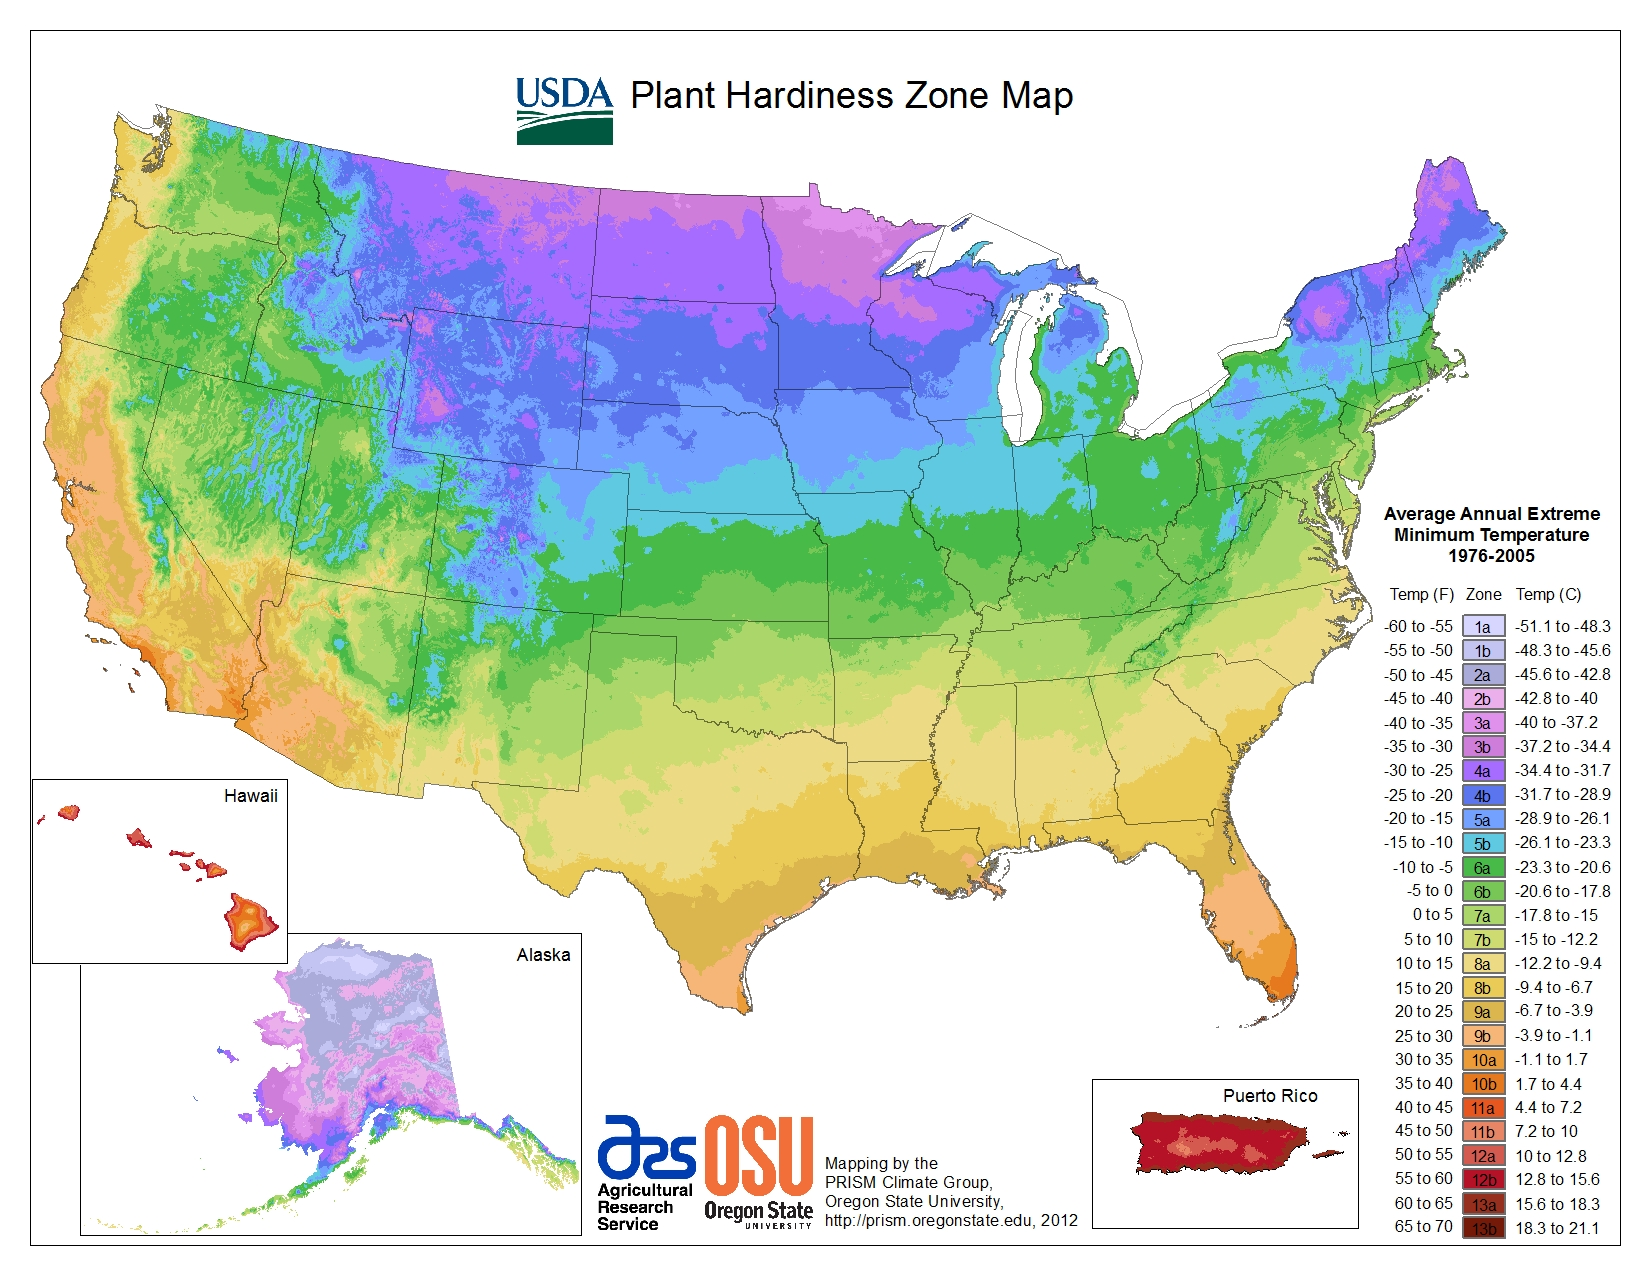
\includegraphics[width=0.95\textwidth]{images/plant-hardiness-half-zones-usa.jpg}
\end{figure}

\end{frame}


%------------------------------------------%
% Introduction
%------------------------------------------%
%
%\begin{frame}{The Wild Story of How We Got Here and How We Achieve the Dream}
%
%\begin{figure}
%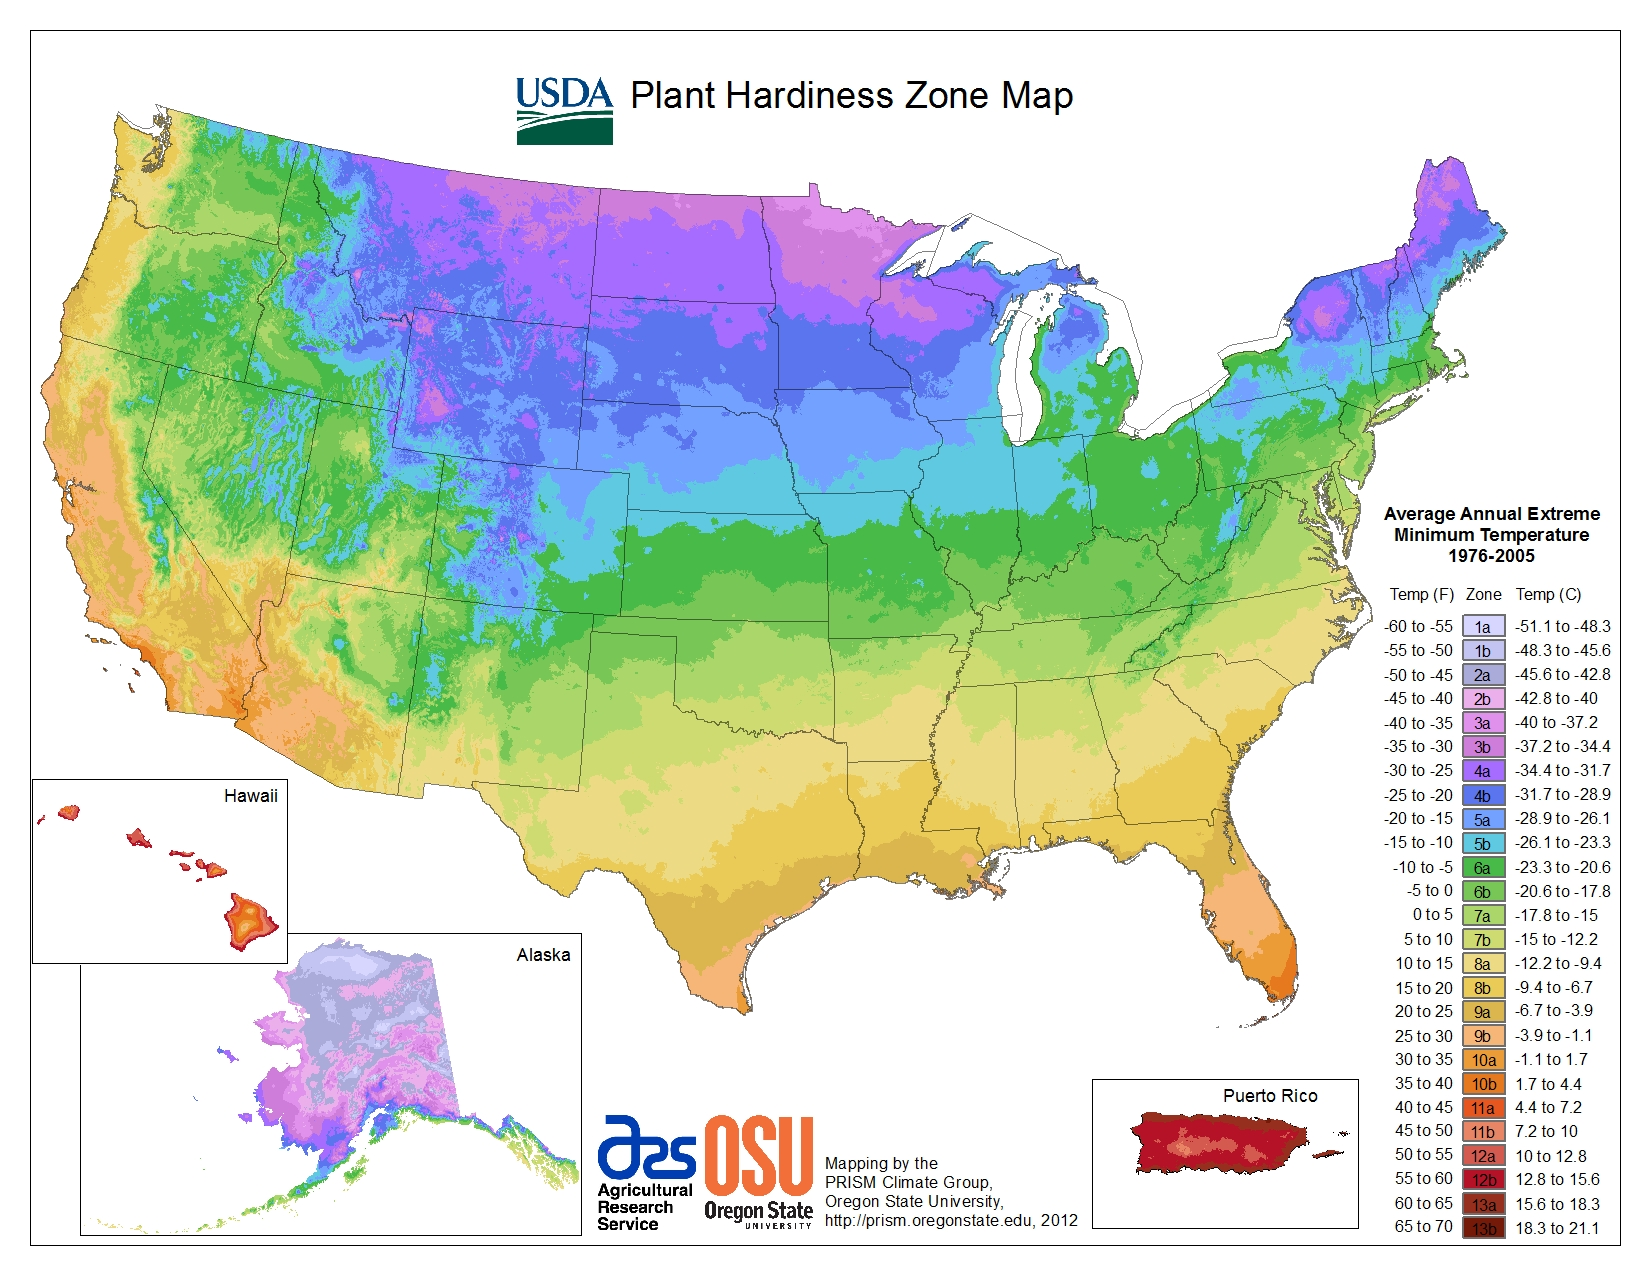
\includegraphics[width=\textwidth]{images/plant-hardiness-half-zones-usa.jpg}
%\end{figure}
%
%\end{frame}


% Neither alcohol nor tobacco is legally listed as a controlled substance.


% MORE Act (CORE Act upon enactment?)

%Marijuana Opportunity Reinvestment and Expungement Act or the MORE Act
%
%This bill decriminalizes marijuana.
%
%Specifically, it removes marijuana from the list of scheduled substances under the Controlled Substances Act and eliminates criminal penalties for an individual who manufactures, distributes, or possesses marijuana.
%
%The bill also makes other changes, including the following:
%
%replaces statutory references to marijuana and marihuana with cannabis,
%requires the Bureau of Labor Statistics to regularly publish demographic data on cannabis business owners and employees,
%establishes a trust fund to support various programs and services for individuals and businesses in communities impacted by the war on drugs,
%imposes an excise tax on cannabis products produced in or imported into the United States and an occupational tax on cannabis production facilities and export warehouses,
%makes Small Business Administration loans and services available to entities that are cannabis-related legitimate businesses or service providers,
%prohibits the denial of federal public benefits to a person on the basis of certain cannabis-related conduct or convictions,
%prohibits the denial of benefits and protections under immigration laws on the basis of a cannabis-related event (e.g., conduct or a conviction),
%establishes a process to expunge convictions and conduct sentencing review hearings related to federal cannabis offenses,
%directs the Government Accountability Office to study the societal impact of state legalization of recreational cannabis,
%directs the National Highway Traffic Safety Administration to study methods for determining whether a driver is impaired by marijuana,
%directs the National Institute for Occupational Safety and Health to study the impact of state legalization of recreational cannabis on the workplace, and
%directs the Department of Education to study the impact of state legalization of recreational cannabis on schools and school-aged children.


%https://www.congress.gov/bill/117th-congress/house-bill/3617

%------------------------------------------%
% Virginia Foxx
%------------------------------------------%

% Virginia Foxx
%voted against the Marijuana Opportunity Reinvestment & Expungement Act (MORE)

% $79,000 and $210,000 in Altria stock


%------------------------------------------%
% Dillon Gentry
%------------------------------------------%


%------------------------------------------%
% Altria
%------------------------------------------%

% Owns stake in Cronos Group, which cultivates high THC cannabis in Canada.

% TODO: DEBUNK!!!!!

% "The overall cost of substance misuse in the United States, which the National Institute on Drug Abuse estimates at $600 billion annually."
% Addressing Youth and Cannabis
%p.24 

% Uncited claim by the National Institute of Drug Abuse.

% How the societal cost of drugs was calculated?

% A 1982 survey of 3,700 households found that the average income of households with at least 1 person who admitted to having ever used marijuana daily (20 days or more in a 30-day period) was 28 percent lower than the average reported income of otherwise similar households.

% Unsubstantiated claim: 

% p.8 Addressing Youth and Cannabis

%https://www.cpear.org/wp-content/uploads/2022/03/CPEAR_Cannabis-Youth-Prevention_Policypaper_.pdf



% "Ensuring youth prevention must be part of cannabis policy reform."
% Cannabis and Youth Use
%https://www.cpear.org/wp-content/uploads/2021/09/Youth-One-Pager-4.pdf

%------------------------------------------%
% Letters from Associations
%------------------------------------------%

%American Trade Association for Cannabis and Hemp
%
%- "Must include a health warning."
%- "...dosage with recommended consumption
%instructions."
%- "...do not make any health claims."
%- "Leading nationwide data collection and public health surveillance."
%- "Edibles prohibited that are shaped like a human, animal, or fruit...
%- "Cannot be on a stick."
%- "Must never be combined or intended to be combined with alcohol or tobacco."
%- "...an excise tax with a rate of 10\% in the first year, growing to 25\% in the fifth year..."
%- "... because of the relative lack of data..."
%Comments on the Cannabis Administration and Opportunity Act
%Coalition for Cannabis Policy, Education, and Regulation
%https://mjbizdaily.com/wp-content/uploads/2021/09/CPEAR-CAOA-Comments.pdf


%------------------------------------------%
% Our Plan
%------------------------------------------%

%This is what we're going to do:
%
%1. Systematically arm ourselves with statistics.
%2. Systematically address all uncited, unsubstantiated claims about cannabis.
%3. Draft our thoughts in our own bills.
%4. Run, vote, and talk to {\bfseries our} representatives.
%5. Speak to everyone about statistics we have discovered and push back against uncited, unsubstantiated claims by returning to step 1.


%------------------------------------------%
% Our Stance
%------------------------------------------%

%1.  Unalienable Right: "the pursuit of Happiness."
%
%2. Any cannabis prohibition is despotic.


%------------------------------------------%
% Seque to conclusion
%------------------------------------------%

%"Tell them about the dream, Martin!"
%-  Mahalia Jackson
% Washington, D.C.'s, Lincoln Memorial Aug. 28, 1963


%------------------------------------------%
% Takeaway
%------------------------------------------%
\section{Takeaway}
\begin{frame}{}

\vspace{0.5\baselineskip}

\begin{center}
\begin{minipage}{3.85in}

% Thank you.

\includegraphics[width=.25in]{images/prayer.png} {\Large \textbf{Thank you for coming.}}\\[-0.75\baselineskip]

\begin{center}
\begin{minipage}{\linewidth}
\begin{Block}{Insight of the Day}

\vspace{0.5\baselineskip}

\begin{itemize}

%\item Words are our most powerful tool.

\item Every piece of the puzzle must be connected.

\vspace{0.5\baselineskip}

\end{itemize}

\end{Block}
\end{minipage}
\end{center}

\vfill

\end{minipage}
\end{center}

\vspace{0.5\baselineskip}

{\large What is on your mind for next week?}\\

\end{frame}


%------------------------------------------%
% Fin.
%------------------------------------------%
\end{document}
